\chapter{Traffic Control}
Traffic control in Linux is realized using a utility named \acs{TC}. It consists of four basic techniques.

\begin{enumerate}
\item \textbf{Shaping}: This is the technique we will be using in order to enforce an upper bandwidth limit. But in general, it is the process of manipulating the bandwidth. It can also be used to smooth out bursts in order to improve the quality of service. Shaping is done on egress traffic.

\item \textbf{Scheduling}: This is the process of staging packets according to a schedule. Like this reordering of packets can be achieved. Scheduling as well happens with egress traffic.

\item \textbf{Policing}: This is the equivalent to shaping but for ingress traffic. It is worth noticing that traffic policing is more limited than traffic shaping, since there is no ingress queue.

\item \textbf{Dropping}: This is a quite primitive approach of just dropping traffic that exceeds a given bandwidth. This is applicable for both ingress and egress traffic.
\end{enumerate}

For our needs, traffic shaping fits best. But since we need to limit ingress traffic as well, and shaping only operates on egress traffic, we need a workaround. More about that in section  \ref{Ingress Traffic}. \acl{TC} on Linux is implemented using three basic building blocks: \acp{QDISC}, classes and filters. They will be discussed in section \ref{TC}.

\newpage
\section{TC} \label{TC}
\acs{TC} is a state of the art traffic control utility that is part of the iproute2 utility package and is by default installed on all \aclp{AP}. It can handle traffic based on any properties that can be found in the \acs{IP}-header, as well as marks that were set using iptables or ipchains.

\subsection{Queuing Disciplines}

A \acs{QDISC} or \acl{QDISC} is the controlling unit that sits between the kernel and the interface. Whenever the kernel wants to send something to an interface, it enqueues it via the \acs{QDISC} attached to the interface. The kernel then immediately tries to get as many packets as possible from the \acs{QDISC} in order to send them to the network adapter driver. The \acs{QDISC} can therefore decide in what manner it allows the kernel to get the packets back in order to send them. Therefore, it is clear that there are very sophisticated egress \acsp{QDISC}, while there is only one very primitive ingress \acs{QDISC}.
\\
As we will see in section \ref{Traffic Shaping}, \acsp{QDISC} can be either classful or classless. If we want to do more than just simple policing or dropping then it is recommended to use classful \acsp{QDISC}, simply because classful \acsp{QDISC} can be configured more precisely, which makes them more powerful.

\subsection{Classes}

Classes are used to configure classful \acsp{QDISC}. They are mostly used to handle a subset of the entire traffic. Which kind of traffic belongs to that subset is determined by classifier filters, which are attached to the parent \acs{QDISC}. Each class has exactly one leaf \acs{QDISC}, but can have multiple non-leaf \acsp{QDISC}, to which there can again be classes attached. Like this classes and \acsp{QDISC} can build up a hierarchy tree, which is then propagated from top to bottom, namely from the root \acs{QDISC} to the leaf \acs{QDISC}.

\subsection{Filters}
There are two main types of filters:
\begin{enumerate}
\item \textbf{Classifiers:} They map traffic based on some metric to a class of a classful \acs{QDISC}, where the traffic is then further handled according to the leaf \acs{QDISC} or filters attached to the class.
\item \textbf{Policers:} They are used to directly manipulate traffic. In our case we use them to redirect traffic from the ingress \acs{QDISC} to a virtual interface (\ac{IFB}). But they can also be used to directly limit the bandwidth, however without the configuration options a classful \acs{QDISC} provides.
\end{enumerate}

\section{Theory}
\subsection{Traffic Shaping}\label{Traffic Shaping}
As previously stated, traffic shaping happens with egress traffic. However, there is a special \acs{QDISC} that is handling ingress traffic. Since this \acs{QDISC} is the only one applicable on ingress traffic, it is called \textit{ingress}. The term \acl{QDISC}, in that case, is a bit misleading, because there is no such thing as an ingress queue. All the other \acsp{QDISC} handle egress traffic and are quite diverse. Each \acs{QDISC} has a shaping algorithm that shapes the traffic passing the corresponding \acs{QDISC}. \acsp{QDISC} can be either classful or classless (the ingress \acs{QDISC} is the latter). Classful \acsp{QDISC} have a shaping algorithm that can handle traffic, which is classified in different classes, differently. Both the classes and the classifiers, which are filters that determine which kind of traffic belongs to which class, are attached to the \acs{QDISC}. Classless \acsp{QDISC} can obviously not handle classes. However they can handle filters, which can either do policing on the traffic or i.e. redirect it to a different interface.

\subsection{Egress Traffic}
To enforce a bandwidth limit per \acs{IP} connection it makes sense to use a classful \acs{QDISC}, because this provides us with the flexibility to configure the classes exactly according to our needs. The best choice for a classful egress \acs{QDISC} that allows us to enforce bandwidth limits, seems to be an \ac{HTB}-\acs{QDISC}, which is based on the \ac{TBF} shaping algorithm. The \acs{TBF} algorithm roughly works as follows: 
\\There is a bucket that holds tokens. Every token corresponds to approximately one byte. Whenever a packet arrives, the \acs{TBF} algorithm tries to consume as many tokens out of the token bucket as there are bytes in the packet. If there are enough tokens, then the packet can be sent at full speed. If there are not enough tokens, then the packet gets enqueued and has to wait until there are again enough tokens in the bucket. The bucket is constantly being filled with tokens at the rate we configured. Like this the bandwidth can be limited in average and at the same time allow short bursts at maximum speed, where the size of these bursts depends on the size of the bucket. It is worth noticing, that the limitation looses in accuracy if the limit is above 1Mbps. But the accuracy loss shouldn't be too severe for our use-case.
More about the \acs{HTB}-\acs{QDISC} can be found in section 9.5.5. of \textit{Linux advanced routing \& traffic control HOWTO}\cite{hubert2002linux}.

\newpage
\subsection{Ingress Traffic} \label{Ingress Traffic}
There is only one \acs{QDISC} that can handle ingress traffic, namely the \textit{ingress} \acs{QDISC}, which is classless. Since it is classless we can't do traffic shaping per \acs{IP} connection as easily as we do it with egress traffic. Therefore we are left with two options:
\begin{enumerate}
\item \textbf{Traffic policing using filters}:
\\With this option we can only use the configuration options \acs{TC}-filters provide. The filters would be directly attached to the ingress \acs{QDISC}. Since these policing options are a bit limited and not as powerful as the shaping options, we are not going to use policing.
\item \textbf{Traffic shaping using virtual interfaces}:
\\The option of using virtual interfaces gives us the same configuration possibilities as we have with egress traffic. At the ingress \acs{QDISC} we simply attach one filter that redirects all the traffic it receives to a virtual interface, on which we then have a \acs{HTB}-\acs{QDISC} and therefore have the same options as we have with the \acs{HTB}-\acs{QDISC} that handles egress traffic. You can think about this the following way: The virtual interface sends the ingress traffic to the host and therefore the ingress traffic becomes egress traffic from the perspective of the virtual interface. Figure \ref{Interface set-up} should make that clearer. Since this option is more powerful, in the sense that we have more shaping options and because using the same egress \acs{QDISC} on the virtual interface as we use on the physical interface gives us the advantage that the entire set-up is more symmetric and therefore easier to understand and debug, this is our option of choice.

\end{enumerate}

\begin{figure}[h]
	\centering
	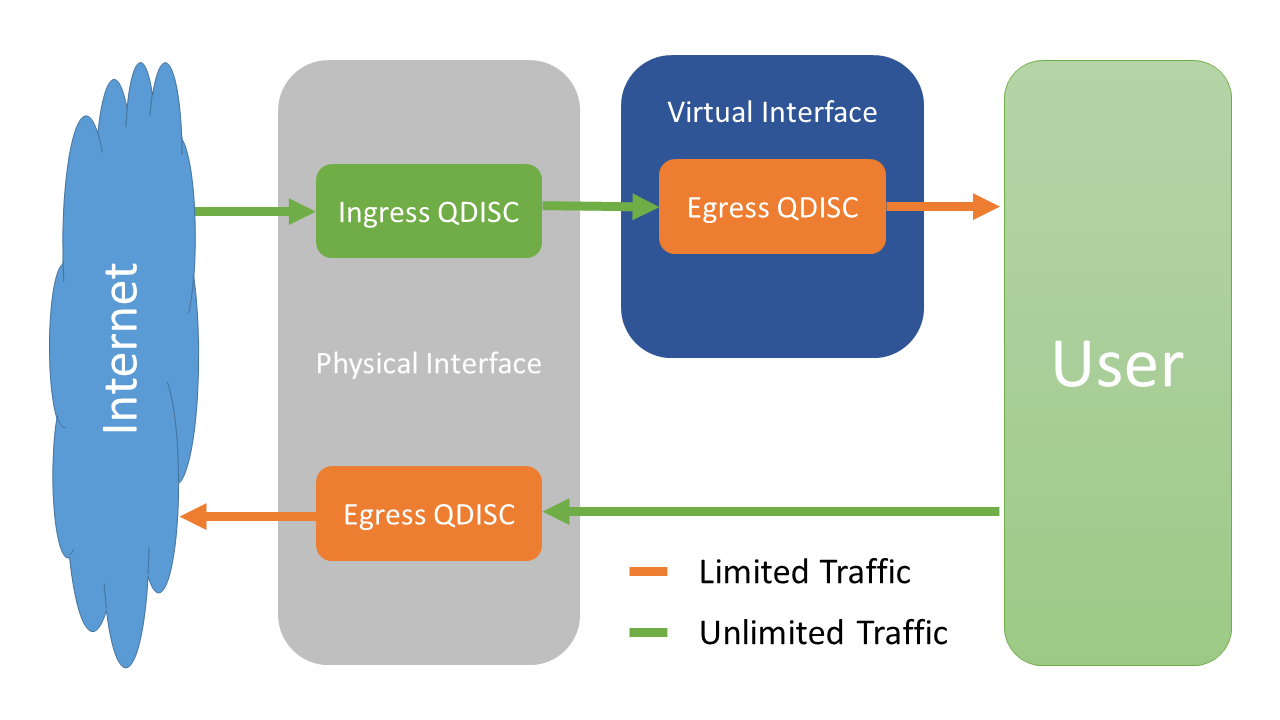
\includegraphics[width=0.9\textwidth]{img/Interface-Setup.png}
	\caption{Interface set-up}
	\label{Interface set-up}
\end{figure}